\documentclass[11pt,a4paper]{article}

\usepackage[utf8]{inputenc}
\usepackage[T1]{fontenc}
\usepackage[english]{babel}
\usepackage[a4paper,margin=2.5cm]{geometry}
\usepackage{hyperref}
\usepackage{xcolor}
\usepackage{listings}
\usepackage{booktabs}
\usepackage{graphicx}
\usepackage{enumitem}
\usepackage{titlesec}
\usepackage{newtxtext}
\usepackage{newtxmath}
\usepackage{tikz}
\usetikzlibrary{positioning,arrows.meta,calc,shapes.multipart}

\hypersetup{
  colorlinks=true,
  linkcolor=black,
  urlcolor=blue!60!black,
  citecolor=blue!60!black,
}

\definecolor{codebg}{RGB}{246,246,246}
\definecolor{codecomment}{RGB}{96,128,96}
\definecolor{codestring}{RGB}{120,80,40}
\definecolor{codekeyword}{RGB}{40,60,160}

\lstset{
  backgroundcolor=\color{codebg},
  basicstyle=\ttfamily\footnotesize,
  breaklines=true,
  commentstyle=\color{codecomment}\itshape,
  keywordstyle=\color{codekeyword}\bfseries,
  stringstyle=\color{codestring},
  frame=single,
  framerule=0pt,
  rulecolor=\color{codebg},
  xleftmargin=8pt,
  xrightmargin=4pt,
  showstringspaces=false,
  tabsize=2,
  captionpos=b,
}

\titlespacing*{\section}{0pt}{14pt}{6pt}
\titlespacing*{\subsection}{0pt}{10pt}{4pt}

% Number paragraphs as "5.1.1.", restarting the paragraph counter at every
% subsection so the test groups read "5.1.1 Diff formatter", etc.
\setcounter{secnumdepth}{4}
\renewcommand{\theparagraph}{\thesubsection.\arabic{paragraph}.}
\makeatletter
\@addtoreset{paragraph}{subsection}
\makeatother

\setlist{topsep=2pt,itemsep=2pt,parsep=0pt}

\setlength{\emergencystretch}{3em}
\hyphenpenalty=200
\tolerance=2000

\title{\textbf{ARC-AGI-2 Agentic Solver Test Suite}\\
\Large{Testing and Validation Project}}
\author{Nagy Dezső\\Számítástechnika IV.\\Sapientia}
\date{April 2026}

\begin{document}
\maketitle
\vspace{2cm}
\tableofcontents
\clearpage
\hrule

\section{Introduction}

\subsection{What is software testing?}

Testing is the practice of running a program against inputs you control and comparing what comes out against what you expected. It is not proof of correctness, a passing suite only says tests our expected assumptions on how the system should behave, but it is the cheapest way to catch the regressions that creep in between changes. When the project starts touching real APIs that cost money, that cheap feedback loop quickly becomes the difference between a solver you can add features to or one nobody dares to touch.

\section{Project Overview}

\subsection{The ARC-AGI-2 benchmark}

ARC-AGI-2 \cite{arcprize} is a visual reasoning benchmark. Each task gives the solver a handful of training pairs of small grids of integers (values 0--9) and asks it to figure out the transformation rule that maps input grids to output grids. The solver then has to apply that rule to a held-out test grid. The grids are small but the rules are diverse: rotations, recolouring, object isolation, symmetry completion, and many things in between. Performance is measured by how many test grids are solved correctly.

\begin{figure}[h]
  \centering
  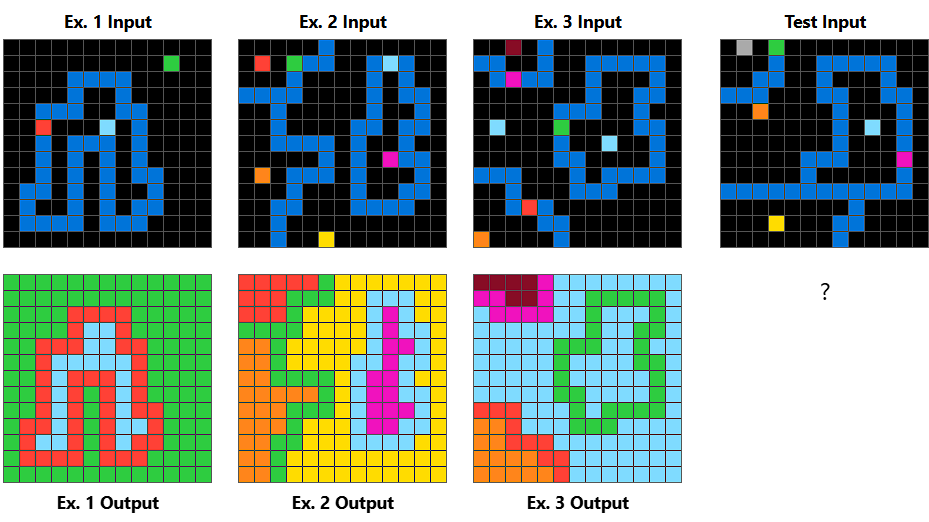
\includegraphics[width=0.8\textwidth]{arc-agi.png}
  \caption{An example of an ARC-AGI task.}
  \label{fig:arc-agi-example}
\end{figure}

\subsection{The base repo and what I changed}

The codebase started as a fork of Confluence Labs' \emph{Saturating ARC-AGI-2} \cite{baserepo}, which holds one of the best performing solvers on the public-evaluation set. That gave me a working solver to build on top of. The pieces I contributed and which the test suite focuses on are:

\begin{itemize}
  \item A pluggable CLI layer: a common \texttt{BaseCLI} protocol with three concrete adapters (Gemini, OpenCode, Junie), so swapping the agent CLI is a single argument change.
  \item A Docker backend sitting alongside the original E2B runner under a shared \texttt{BackendRunner} protocol.
  \item A typed model layer (Pydantic v2) and a refactored, typed orchestrator API.
  \item A streaming log protocol that splits agent stdout into a session log, a transcript, and a human-readable Markdown rendering, with per-call cost tracking.
  \item The full test suite with multiple tiers of unit, functional and integration tests.
\end{itemize}

\subsection{Why testing is needed}

The solver assigns multiple agents for each task, each running in its own sandbox, each calling a remote LLM API dozens of times. A single full evaluation run hits the API budget hard. Without tests, every refactor is a coin flip: you might find out at hour eight that a typo in the cost aggregator silently double-counted half the runs. With tests, the parser, the diff formatter, the orchestrator's resume logic, and the backend's output routing are all pinned down before any of that runs. The functional layer in particular catches the kind of bug that only shows up under concurrency: ordering issues, missing semaphore acquisitions, exception handling that drops one agent and crashes the rest.

\subsection{Architecture}


\begin{figure}[h]
  \centering
  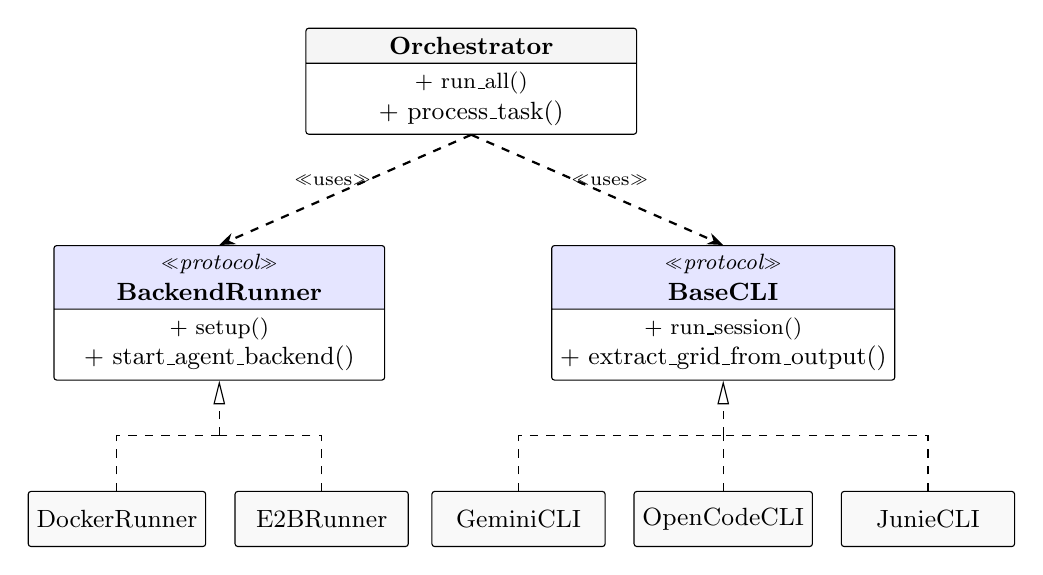
\begin{tikzpicture}[
      font=\small,
      every node/.style={align=center},
      iface/.style={
        draw, rectangle split, rectangle split parts=2,
        rectangle split part fill={blue!10, white},
        minimum width=42mm, inner sep=3pt, rounded corners=1pt,
      },
      cls/.style={
        draw, rectangle split, rectangle split parts=2,
        rectangle split part fill={gray!8, white},
        minimum width=42mm, inner sep=3pt, rounded corners=1pt,
      },
      concrete/.style={
        draw, rectangle, fill=gray!5,
        minimum width=22mm, minimum height=7mm,
        inner sep=3pt, rounded corners=1pt,
      },
      uses/.style={-{Stealth[length=2mm]}, dashed, thick},
      realize/.style={-{Triangle[open,length=3mm]}, dashed},
    ]

    % Orchestrator at top centre
    \node[cls] (orch) {%
      \textbf{Orchestrator}
      \nodepart{two}\footnotesize
      + run\_all()\\
      + process\_task()
    };

    % Protocols, well separated horizontally
    \node[iface, below=14mm of orch, xshift=-32mm] (be) {%
      \footnotesize\textit{«protocol»}\\\textbf{BackendRunner}
      \nodepart{two}\footnotesize
      + setup()\\
      + start\_agent\_backend()
    };
    \node[iface, below=14mm of orch, xshift=32mm] (cli) {%
      \footnotesize\textit{«protocol»}\\\textbf{BaseCLI}
      \nodepart{two}\footnotesize
      + run\_session()\\
      + extract\_grid\_from\_output()
    };

    % Concrete backends — two boxes under BackendRunner
    \node[concrete, below=14mm of be, xshift=-13mm] (docker) {DockerRunner};
    \node[concrete, below=14mm of be, xshift=13mm]  (e2b)    {E2BRunner};

    % Concrete CLIs — three boxes under BaseCLI
    \node[concrete, below=14mm of cli, xshift=-26mm] (gem) {GeminiCLI};
    \node[concrete, below=14mm of cli]               (opc) {OpenCodeCLI};
    \node[concrete, below=14mm of cli, xshift=26mm]  (jun) {JunieCLI};

    % Join coordinates so the realisation arrows form a clean fork
    \coordinate (beJoin)  at ($(be.south)+(0,-7mm)$);
    \coordinate (cliJoin) at ($(cli.south)+(0,-7mm)$);

    % Orchestrator → protocols (dependencies, dashed open arrow)
    \draw[uses] (orch.south) -- node[pos=0.55, above, font=\scriptsize]{«uses»} (be.north);
    \draw[uses] (orch.south) -- node[pos=0.55, above, font=\scriptsize]{«uses»} (cli.north);

    % Realisations: concrete -> join point -> protocol (single triangle arrow into protocol)
    \draw[dashed] (docker.north) |- (beJoin);
    \draw[dashed] (e2b.north)    |- (beJoin);
    \draw[realize] (beJoin) -- (be.south);

    \draw[dashed] (gem.north) |- (cliJoin);
    \draw[dashed] (opc.north) -- (cliJoin);
    \draw[dashed] (jun.north) |- (cliJoin);
    \draw[realize] (cliJoin) -- (cli.south);

  \end{tikzpicture}
  \caption{Class diagram of the pluggable layers.}
  \label{fig:uml}
\end{figure}

At runtime, after parsing the command line arguments, the Orchestrator schedules one coroutine per ARC task. Each of them assings agents through a API call semaphore, and every agent goes through the chosen BackendRunner into a sandbox where the agent runner controls the chosen CLI for some number of refinement turns.

\section{Testing Framework}

\subsection{Pytest}

I picked \texttt{pytest} for the following reasons:

\begin{itemize}
  \item It's easy to use. Plain \texttt{assert} statements, and the test body reads like the hypothesis it encodes.
  \item It's one of the most widely used Python testing libraries, and a particularly natural fit for a project this size. It has support for asynchronous tests with \texttt{pytest-asyncio} and mocking with \texttt{pytest-mock} so I didn't have to write any boilerplate code.
  \item Fixtures take the pain out of test environment setup. Defining a temporary workspace, a mock task JSON, and a fully wired-up mock CLI in one file once and using them in later tests rather than copy-pasting setup code into every file.
  \item I like how the decorators make intent visible at a glance. \texttt{@pytest.mark.asyncio}, \texttt{@pytest.mark.parametrize}, and the \texttt{unit} / \texttt{functional} / \texttt{integration} markers all show up next to the test they describe, not in some external configuration.
\end{itemize}

\subsection{Installation}

Clone, install dev dependencies, run the suite:

\begin{lstlisting}[language=bash]
git clone https://github.com/NagyDezso/arc-agi-2.git
cd arc-agi-2
uv sync --group dev

uv run pytest tests/unit
uv run pytest tests/functional
uv run pytest tests/integration   # needs API keys and Docker access
\end{lstlisting}

\section{Repository structure}

The repository structure is as follows:

\begin{lstlisting}[caption={Top-level layout.}]
arc-agi-2/
|-- src/                              # implementation
|-- tests/                            # the suite
|-- data/                             # ARC-AGI-2 puzzle JSONs
|-- pyproject.toml                    # pytest + ruff config
|-- .github/workflows/tests.yml       # CI
|-- main.py                           # entry point
\end{lstlisting}

\subsection{Puzzle Data}

The \texttt{data/} folder holds two JSON files from the ARC Prize: the challenges file and the matching solutions file (\texttt{arc-agi\_evaluation\_challenges.json} and \texttt{arc-agi\_evaluation\_solutions.json}). The schema, in one line:

\begin{lstlisting}[caption={Task schema.}]
{ "<task_id>": { "train": [ { "input": [[...]], "output": [[...]] } ],
                  "test":  [ { "input": [[...]] } ] } }
\end{lstlisting}

Every \texttt{input} and \texttt{output} is a 2D list of integers in the range 0--9. The solver only sees the \texttt{train} pairs and the \texttt{test} inputs; the solutions file is only used at scoring time.

For testing, none of this real data is required. Tests build minimal task dictionaries on the fly via the \texttt{mock\_task\_data} fixture, with a single 2$\times$2 train pair and a single 2$\times$2 test input. That is enough to exercise the agent loop, the orchestrator state machine, and every code path that depends on task structure.

\subsection{Test directory layout}

\begin{lstlisting}[caption={Tests groupings}]
tests/
|-- conftest.py                       # shared fixtures
|-- unit/
|   |-- test_agent_runner.py
|   |-- test_cli_impl.py
|   `-- test_docker_runner.py
|-- functional/
|   |-- test_agent_runner_errors.py
|   `-- test_orchestrator.py
`-- integration/
    |-- test_cli_integration.py
    `-- test_docker_integration.py
\end{lstlisting}

\subsection{Shared fixtures}

\texttt{tests/conftest.py} defines five fixtures every test in the suite can pull in:

\begin{itemize}
  \item \texttt{mock\_task\_data}: a minimal task dict.
    \\ \texttt{"train": [{"input": [[0, 0], [0, 0]], "output": [[1, 1], [1, 1]]}]}
    \\ \texttt{"test": [{"input": [[0, 0], [0, 0]]}]}.
  \item \texttt{temp\_workspace}: a \texttt{tempfile.TemporaryDirectory} yielded as a \texttt{Path}, cleaned up automatically.
  \item \texttt{mock\_raw\_task\_file}: writes \texttt{mock\_task\_data} to a \texttt{task.json} inside \texttt{temp\_workspace} and returns the path.
  \item \texttt{mock\_test\_prompt}: a constant string used by tests that need a non-empty prompt.
  \item \texttt{mock\_cli\_impl}: a \texttt{MagicMock} configured with defaults (zero cost, empty session output).
\end{itemize}

\section{Testing Suite}

\subsection{Unit tests}

Pure functions and small components, no I/O beyond a temporary file.

\paragraph{Diff formatter:}
The function the agent loop uses to know what went wrong on its last attempt.
\begin{description}[leftmargin=10pt,style=nextline,itemsep=6pt,parsep=1pt,font=\normalfont]
  \item[\texttt{test\_format\_diff}]
    \textbf{Description:} Verifies the diff formatter highlights mismatched cells correctly. \\
    \textbf{Input:} Two grids differing in one cell. \\
    \textbf{Expected:} Diff string naming the coordinate (\texttt{(0,1): 2 -> 0}) and printing both grids.
  \item[\texttt{test\_format\_diff\_shape\_mismatch}]
    \textbf{Description:} Verifies the diff formatter handles shape mismatches gracefully instead of crashing on a per-cell diff. \\
    \textbf{Input:} Grids of different shapes. \\
    \textbf{Expected:} A clear shape-mismatch message, no per-cell diff attempted.
\end{description}

\paragraph{Transform validator:}
Decides whether the agent's submitted Python passes the training examples.
\begin{description}[leftmargin=10pt,style=nextline,itemsep=6pt,parsep=1pt,font=\normalfont]
  \item[\texttt{test\_run\_transform\_success}]
    \textbf{Description:} Verifies that a correct transform passes against scripted training pairs. \\
    \textbf{Input:} Correct \texttt{transform.py} function and matching training examples. \\
    \textbf{Expected:} \texttt{(True, "All training examples pass.", fn)}.
  \item[\texttt{test\_test\_transform\_failure}]
    \textbf{Description:} Verifies that a wrong transform produces the feedback string the agent loop echoes back to the LLM. \\
    \textbf{Input:} A wrong \texttt{transform.py} function. \\
    \textbf{Expected:} \texttt{(False, msg, None)} where \texttt{msg} starts with \texttt{Value mismatch}.
\end{description}

\paragraph{CLI output parsers:}
Pulls the final grid out of three different agent-CLI transcript formats.
\begin{description}[leftmargin=10pt,style=nextline,itemsep=6pt,parsep=1pt,font=\normalfont]
  \item[\texttt{test\_gemini\_extract\_grid\_from\_output}]
    \textbf{Description:} Verifies the Gemini parser pulls a grid out of both event types it can appear in. \\
    \textbf{Input:} Gemini \texttt{tool\_result} or \texttt{write\_file} carrying a grid. \\
    \textbf{Expected:} Parsed Python list.
  \item[\texttt{test\_opencode\_extract\_grid\_from\_output}]
    \textbf{Description:} Verifies the OpenCode parser handles its different event format. \\
    \textbf{Input:} OpenCode \texttt{text} event or \texttt{write} tool call carrying a grid. \\
    \textbf{Expected:} Parsed Python list.
\end{description}

\paragraph{Readable-log writers:}
Builds a Markdown output of each agent run.
\begin{description}[leftmargin=10pt,style=nextline,itemsep=6pt,parsep=1pt,font=\normalfont]
  \item[\texttt{test\_gemini\_write\_readable\_log\_handles\_split\_deltas}]
    \textbf{Description:} Verifies streamed delta messages get stitched back into one piece of text. \\
    \textbf{Input:} Two delta-message events \texttt{"Hello "} and \texttt{"world"}. \\
    \textbf{Expected:} Buffer holds exactly \texttt{"Hello world"}, no duplicates.
  \item[\texttt{test\_opencode\_write\_readable\_log\_includes\_tool\_result}]
    \textbf{Description:} Verifies tool calls render with the full Markdown layout (header and result block). \\
    \textbf{Input:} OpenCode \texttt{tool\_use} for \texttt{bash}. \\
    \textbf{Expected:} Markdown contains \texttt{**Tool: bash**} and \texttt{**Tool Result:**}.
\end{description}

\paragraph{Docker output routing:}
Splits agent stdout into the right files.
\begin{description}[leftmargin=10pt,style=nextline,itemsep=6pt,parsep=1pt,font=\normalfont]
  \item[\texttt{test\_docker\_runner\_routes\_status\_and\_transcript\_lines}]
    \textbf{Description:} Verifies each kind of stdout line lands in its intended destination. \\
    \textbf{Input:} \texttt{Status} and \texttt{Transcript} events plus an unknown-type line. \\
    \textbf{Expected:} \texttt{Status} hits session log and logger, \texttt{Transcript} hits transcript file with no envelope, unknown lines are logged as warnings.
\end{description}

\subsection{Functional tests}

Real orchestrator and agent runner, mocked external dependencies (Docker, HTTP, the LLM CLI). These tests cover the multi-agent state machine.

\paragraph{Agent-loop error handling:}
\begin{description}[leftmargin=10pt,style=nextline,itemsep=6pt,parsep=1pt,font=\normalfont]
  \item[\texttt{test\_run\_agent\_should\_stop\_on\_fatal\_errors}]
    \textbf{Description:} Verifies the agent loop aborts immediately on fatal errors instead of burning its full iteration budget. \\
    \textbf{Input:} 5 parametrised fatal errors (\texttt{ModelNotFoundError}, \texttt{Invalid model}, \texttt{QuotaExceeded}, \texttt{Access denied}, \texttt{Requested entity was not found}). \\
    \textbf{Expected:} \texttt{run\_session} called exactly once, error preserved in \texttt{stderr}.
\end{description}

\paragraph{Score aggregation:}
\begin{description}[leftmargin=10pt,style=nextline,itemsep=6pt,parsep=1pt,font=\normalfont]
  \item[\texttt{test\_process\_task\_aggregates\_multi\_agent\_multi\_test\_results}]
    \textbf{Description:} Verifies cost, token and elapsed-time aggregation across multiple agents and tests. \\
    \textbf{Input:} 2 agents $\times$ 2 tests, one empty grid. \\
    \textbf{Expected:} Correct sum of costs / tokens / elapsed time, \texttt{score.submitted == 2}, persisted JSON has all four agent IDs.
  \item[\texttt{test\_process\_task\_whole\_task\_counts\_submissions\_from\_multiple\_test\_indexes}]
    \textbf{Description:} Verifies whole-task mode counts attempts spanning distinct test indices. \\
    \textbf{Input:} Whole-task mode with attempts spanning two \texttt{test\_index} values. \\
    \textbf{Expected:} \texttt{score.submitted == 2}, \texttt{readable.md} generated.
  \item[\texttt{test\_process\_task\_handles\_empty\_attempts}]
    \textbf{Description:} Verifies an empty attempt list is not counted as a submission. \\
    \textbf{Input:} Agent returns \texttt{attempts=[]}. \\
    \textbf{Expected:} \texttt{score.submitted == 0}, backend still called once.
\end{description}

\paragraph{Failure isolation:}
\begin{description}[leftmargin=10pt,style=nextline,itemsep=6pt,parsep=1pt,font=\normalfont]
  \item[\texttt{test\_process\_task\_persists\_exception\_as\_agent\_error}]
    \textbf{Description:} Verifies a single failing agent does not break its sibling agents. \\
    \textbf{Input:} One agent raises \texttt{RuntimeError}. \\
    \textbf{Expected:} Failed agent recorded with \texttt{error} field, \texttt{error.log} written, surviving agent unaffected.
  \item[\texttt{test\_run\_all\_continues\_after\_process\_task\_crash}]
    \textbf{Description:} Verifies a single task crash does not abort the entire run. \\
    \textbf{Input:} \texttt{process\_task} raises for one task. \\
    \textbf{Expected:} Run finishes, \texttt{summary.json} contains only the successful task.
\end{description}

\paragraph{Concurrency \& resume:}
\begin{description}[leftmargin=10pt,style=nextline,itemsep=6pt,parsep=1pt,font=\normalfont]
  \item[\texttt{test\_process\_task\_respects\_backend\_semaphore\_concurrency\_limit}]
    \textbf{Description:} Verifies the concurrency semaphore actually serialises agent dispatch. \\
    \textbf{Input:} 3 agents through a semaphore with a limit of 1. \\
    \textbf{Expected:} \texttt{backend.max\_active == 1} (serialised).
  \item[\texttt{test\_run\_all\_skips\_completed\_tasks\_and\_writes\_summary}]
    \textbf{Description:} Verifies resume logic skips already-finished tasks and still reports them in the summary. \\
    \textbf{Input:} Resume dir already contains \texttt{task\_a.json}, list \texttt{[a,b,c]}, \texttt{limit=1}. \\
    \textbf{Expected:} Only \texttt{task\_b} processed, \texttt{summary.json} reports all three in totals.
\end{description}

\paragraph{End-to-end (mock backend):}
\begin{description}[leftmargin=10pt,style=nextline,itemsep=6pt,parsep=1pt,font=\normalfont]
  \item[\texttt{test\_process\_task\_integration}]
    \textbf{Description:} Smoke-tests the full pipeline against a mock backend, checking every artefact lands on disk. \\
    \textbf{Input:} \texttt{MockBackend} returns one attempt. \\
    \textbf{Expected:} \texttt{score.submitted == 1}, run dir contains \texttt{task\_results/*.json} and per-agent logs (\texttt{session.log}, \texttt{transcript.jsonl}, \texttt{readable.md}, \texttt{attempts.jsonl}).
\end{description}

\subsection{Integration tests}

Real credentials, real services. Skipped in CI. Can be run locally with provided API keys to detect external changes.

\paragraph{API smoke tests:}
\begin{description}[leftmargin=10pt,style=nextline,itemsep=6pt,parsep=1pt,font=\normalfont]
  \item[\texttt{test\_gemini\_real\_usage}, \texttt{test\_opencode\_real\_usage}, \texttt{test\_junie\_real\_usage}]
    \textbf{Description:} Verifies each adapter actually talks to its live API. \\
    \textbf{Input:} Real workspace and a live API call. \\
    \textbf{Expected:} \texttt{turns > 0} and a non-zero token count.
\end{description}

\paragraph{Bad-model failure:}
\begin{description}[leftmargin=10pt,style=nextline,itemsep=6pt,parsep=1pt,font=\normalfont]
  \item[\texttt{test\_gemini\_bad\_model\_failure}, \texttt{test\_opencode\_bad\_model\_failure}]
    \textbf{Description:} Verifies adapters fail gracefully on an invalid model rather than throwing. \\
    \textbf{Input:} Invalid model name. \\
    \textbf{Expected:} Graceful return, error in \texttt{stderr}, no exception escapes the adapter.
\end{description}

\paragraph{Docker integration:}
\begin{description}[leftmargin=10pt,style=nextline,itemsep=6pt,parsep=1pt,font=\normalfont]
  \item[\texttt{test\_docker\_opencode\_agent}]
    \textbf{Description:} Verifies a real Docker container can run an OpenCode session end-to-end. \\
    \textbf{Input:} Real container running an OpenCode session. \\
    \textbf{Expected:} \texttt{session.log} exists and contains the start marker.
  \item[\texttt{test\_docker\_run\_agent\_failure}]
    \textbf{Description:} Verifies the Docker backend handles a misconfigured run without crashing. \\
    \textbf{Input:} Real container with a bad config. \\
    \textbf{Expected:} No crash, no attempts submitted, error reaches \texttt{stderr}.
\end{description}

\section{Continuous integration}

The project has a CI workflow that runs on every push and every pull request against \texttt{main}. If the testing suite fails, the build will fail as well.

\begin{lstlisting}[language=bash,caption={\texttt{.github/workflows/tests.yml} (abbreviated).}]
name: tests
on:
  push:        { branches: [main] }
  pull_request:{ branches: [main] }

jobs:
  test:
    runs-on: ubuntu-latest
    steps:
      - uses: actions/checkout@v4
      - uses: astral-sh/setup-uv@v3
      - run: uv sync --group dev
      - run: uv run ruff check .
      - run: uv run pytest tests/unit tests/functional
      # Integration tests are intentionally skipped as they need API keys and Docker access
\end{lstlisting}

\section{Summary}

The test suite covers the parts of the system where regressions are silent and expensive: the diff formatter that decides whether an agent's transform is correct, the parsers that pull a grid out of three different CLI output formats, the orchestrator's state machine across multi-agent and multi-test inputs, the resume logic that picks up partial runs, and the Docker backend's output routing. The functional tests in particular cover concurrency-sensitive code paths: semaphore contention, exception propagation, partial failures. Preventing these errors reduces the risk of failed runs, that could be costly.

\bigskip
\hrule
\bigskip

\begin{thebibliography}{9}
  \bibitem{arcprize} ARC Prize 2025. \url{https://arcprize.org/}
  \bibitem{baserepo} Confluence Labs, \emph{Saturating ARC-AGI-2}. \url{https://github.com/confluence-labs/arc-agi-2}
\end{thebibliography}

\end{document}
